\subsection{Organigrama}

Contrariamente a la estructura jerárquica lineal propia de la gran mayoría de las corporaciones, The Walt Disney Company estructura su organigrama basándose en los procesos. De esta manera, se crea una red inminentemente sinérgica entre los diferentes sectores del núcleo de operaciones, que dependen de sus sectores colindantes y, a su vez, son dependencias del trabajo de ellos.

\begin{figure}[!htb]
\centering
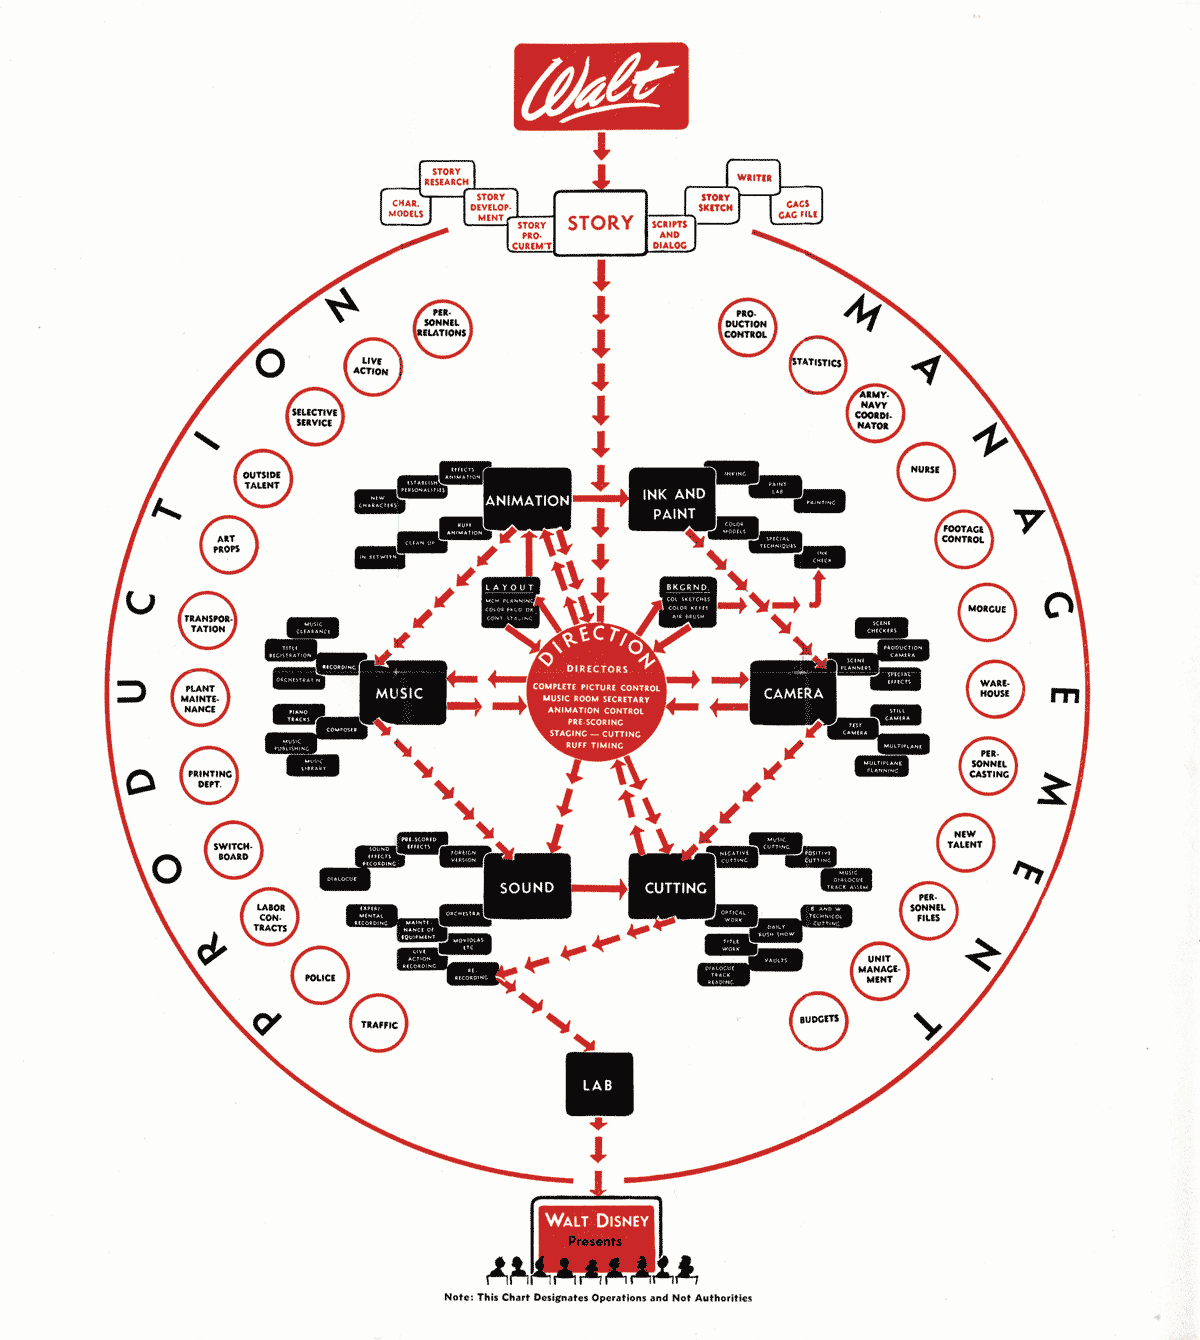
\includegraphics[scale=0.3]{organigramadisney.png}
\caption{\label{fig:frog}Organigrama The Walt Disney Company (1943)}
\end{figure}

El organigrama más conocido de la empresa fue publicado en 1943 (Hirasuna, 2009) y muestra cómo cada una de las posiciones del staff son absolutamente necesarias para mantener activo el flujo del trabajo desde que la historia llega al equipo directivo cinematográfico desde los guionistas hasta que se lleva al público en la gran pantalla.